%35
\subsection{Új elemek sorba helyezése (enqueue)}
\begin{frame}
  \begin{columns}[c]
    \column{0.4\textwidth}
      \scriptsize
      \begin{exampleblock}{\textattachfile{sor2.cpp}{sor2.cpp}}
        \meret{7}
        \vspace{-.2cm}
        \lstinputlisting[style=cpp,linerange={4-24},numbers=left,firstnumber=4]{sor2.cpp}
        \vspace{-.2cm}
      \end{exampleblock}
    \column{0.55\textwidth}
      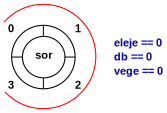
\includegraphics[width=\textwidth]{sor/sor01.pdf}
  \end{columns}
\end{frame}

%36
\begin{frame}
  \begin{columns}[c]
    \column{0.4\textwidth}
      \scriptsize
      \begin{exampleblock}{\textattachfile{sor2.cpp}{sor2.cpp}}
        \meret{7}
        \vspace{-.2cm}
        \lstinputlisting[style=cpp,linerange={4-24},numbers=left,firstnumber=4]{sor2.cpp}
        \vspace{-.2cm}
      \end{exampleblock}
    \column{0.55\textwidth}
      \includegraphics[width=\textwidth]{sor/sor02.pdf}
  \end{columns}
\end{frame}

%37
\begin{frame}
  \begin{columns}[c]
    \column{0.4\textwidth}
      \scriptsize
      \begin{exampleblock}{\textattachfile{sor2.cpp}{sor2.cpp}}
        \meret{7}
        \vspace{-.2cm}
        \lstinputlisting[style=cpp,linerange={4-24},numbers=left,firstnumber=4]{sor2.cpp}
        \vspace{-.2cm}
      \end{exampleblock}
    \column{0.55\textwidth}
      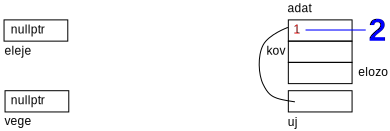
\includegraphics[width=\textwidth]{sor/sor03.pdf}
  \end{columns}
\end{frame}

%38
\begin{frame}
  \begin{columns}[c]
    \column{0.4\textwidth}
      \scriptsize
      \begin{exampleblock}{\textattachfile{sor2.cpp}{sor2.cpp}}
        \meret{7}
        \vspace{-.2cm}
        \lstinputlisting[style=cpp,linerange={4-24},numbers=left,firstnumber=4]{sor2.cpp}
        \vspace{-.2cm}
      \end{exampleblock}
    \column{0.55\textwidth}
      \includegraphics[width=\textwidth]{sor/sor04.pdf}
  \end{columns}
\end{frame}

%39
\begin{frame}
  \begin{columns}[c]
    \column{0.4\textwidth}
      \scriptsize
      \begin{exampleblock}{\textattachfile{sor2.cpp}{sor2.cpp}}
        \meret{7}
        \vspace{-.2cm}
        \lstinputlisting[style=cpp,linerange={4-24},numbers=left,firstnumber=4]{sor2.cpp}
        \vspace{-.2cm}
      \end{exampleblock}
    \column{0.55\textwidth}
      \includegraphics[width=\textwidth]{sor/sor05.pdf}
  \end{columns}
\end{frame}

%40
\begin{frame}
  \begin{columns}[c]
    \column{0.4\textwidth}
      \scriptsize
      \begin{exampleblock}{\textattachfile{sor2.cpp}{sor2.cpp}}
        \meret{7}
        \vspace{-.2cm}
        \lstinputlisting[style=cpp,linerange={4-24},numbers=left,firstnumber=4]{sor2.cpp}
        \vspace{-.2cm}
      \end{exampleblock}
    \column{0.55\textwidth}
      \includegraphics[width=\textwidth]{sor/sor06.pdf}
  \end{columns}
\end{frame}

%41
\begin{frame}
  \begin{columns}[c]
    \column{0.4\textwidth}
      \scriptsize
      \begin{exampleblock}{\textattachfile{sor2.cpp}{sor2.cpp}}
        \meret{7}
        \vspace{-.2cm}
        \lstinputlisting[style=cpp,linerange={4-24},numbers=left,firstnumber=4]{sor2.cpp}
        \vspace{-.2cm}
      \end{exampleblock}
    \column{0.55\textwidth}
      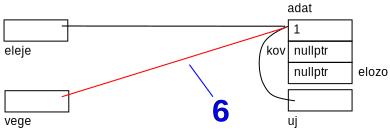
\includegraphics[width=\textwidth]{sor/sor07.pdf}
  \end{columns}
\end{frame}

%42
\begin{frame}
  \begin{columns}[c]
    \column{0.4\textwidth}
      \scriptsize
      \begin{exampleblock}{\textattachfile{sor2.cpp}{sor2.cpp}}
        \meret{7}
        \vspace{-.2cm}
        \lstinputlisting[style=cpp,linerange={4-24},numbers=left,firstnumber=4]{sor2.cpp}
        \vspace{-.2cm}
      \end{exampleblock}
    \column{0.55\textwidth}
      \includegraphics[width=\textwidth]{sor/sor08.pdf}
  \end{columns}
\end{frame}

%43
\begin{frame}
  \begin{columns}[c]
    \column{0.4\textwidth}
      \scriptsize
      \begin{exampleblock}{\textattachfile{sor2.cpp}{sor2.cpp}}
        \meret{7}
        \vspace{-.2cm}
        \lstinputlisting[style=cpp,linerange={4-24},numbers=left,firstnumber=4]{sor2.cpp}
        \vspace{-.2cm}
      \end{exampleblock}
    \column{0.55\textwidth}
      \includegraphics[width=\textwidth]{sor/sor09.pdf}
  \end{columns}
\end{frame}

%44
\begin{frame}
  \begin{columns}[c]
    \column{0.4\textwidth}
      \scriptsize
      \begin{exampleblock}{\textattachfile{sor2.cpp}{sor2.cpp}}
        \meret{7}
        \vspace{-.2cm}
        \lstinputlisting[style=cpp,linerange={4-24},numbers=left,firstnumber=4]{sor2.cpp}
        \vspace{-.2cm}
      \end{exampleblock}
    \column{0.55\textwidth}
      
\includegraphics[width=\textwidth]{sor/sor10.pdf}
  \end{columns}
\end{frame}

%45
\begin{frame}
  \begin{columns}[c]
    \column{0.4\textwidth}
      \scriptsize
      \begin{exampleblock}{\textattachfile{sor2.cpp}{sor2.cpp}}
        \meret{7}
        \vspace{-.2cm}
        \lstinputlisting[style=cpp,linerange={4-24},numbers=left,firstnumber=4]{sor2.cpp}
        \vspace{-.2cm}
      \end{exampleblock}
    \column{0.55\textwidth}
      \includegraphics[width=\textwidth]{sor/sor11.pdf}
  \end{columns}
\end{frame}

%46
\begin{frame}
  \begin{columns}[c]
    \column{0.4\textwidth}
      \scriptsize
      \begin{exampleblock}{\textattachfile{sor2.cpp}{sor2.cpp}}
        \meret{7}
        \vspace{-.2cm}
        \lstinputlisting[style=cpp,linerange={4-24},numbers=left,firstnumber=4]{sor2.cpp}
        \vspace{-.2cm}
      \end{exampleblock}
    \column{0.55\textwidth}
      \includegraphics[width=\textwidth]{sor/sor12.pdf}
  \end{columns}
\end{frame}

%47
\begin{frame}
  \begin{columns}[c]
    \column{0.4\textwidth}
      \scriptsize
      \begin{exampleblock}{\textattachfile{sor2.cpp}{sor2.cpp}}
        \meret{7}
        \vspace{-.2cm}
        \lstinputlisting[style=cpp,linerange={4-24},numbers=left,firstnumber=4]{sor2.cpp}
        \vspace{-.2cm}
      \end{exampleblock}
    \column{0.55\textwidth}
      \includegraphics[width=\textwidth]{sor/sor13.pdf}
  \end{columns}
\end{frame}

%48
\begin{frame}
  \begin{columns}[c]
    \column{0.4\textwidth}
      \scriptsize
      \begin{exampleblock}{\textattachfile{sor2.cpp}{sor2.cpp}}
        \meret{7}
        \vspace{-.2cm}
        \lstinputlisting[style=cpp,linerange={4-24},numbers=left,firstnumber=4]{sor2.cpp}
        \vspace{-.2cm}
      \end{exampleblock}
    \column{0.55\textwidth}
      \includegraphics[width=\textwidth]{sor/sor14.pdf}
  \end{columns}
\end{frame}